\section{Anexo: Ejemplos}
\subsection{M/M/1}
Supongamos que en una estación existe un sólo servidor que llegan aproximadamente 45 clientes por hora. Se atiende a 60 clients por ahora aproximadamente. Los clientes esperan de promedio 3 minutos en la cola. \\ \\
Conocemos los siguientes datos:
$$\lambda=45 \frac{clientes}{hora}= \frac{45}{60}\frac{clientes}{minutos}$$
$$ \mu = 60 \frac{clientes}{hora} = 1 \frac{clientes}{minutos} $$
$$ W_q = 3 ~ minutos $$
\begin{enumerate}
	\item Tiempo promedio que un cliente pasa en el sistema. \\
	Para calcular el tiempo promedio que un cliente pasa en el sistema ($W_s$). Lo podemos calcular a partir de las fórmulas de esta sección, $W_1$ y $\mu$.
	$$ W_s=W_q+\frac{1}{\mu}=3+1=4 ~ minutos $$ \\
	Es decir, en promedio un cliente pasa 4 minutos en el sistema: 3 minutos apsa esperando en la cola, y un minuto en el servicio.
	\item Para calcular el número de clientes en la cola ($L_q$), usamos la fórmula de esta sección, $L_q=\lambda W_q$. 
	$$ L_q=\lambda W_q = 0.75 \frac{clientes}{minutos} 3 ~ minutos=2.25 ~ clientes$$
	Puede haber más de dos clientes en la cola.
	\item Para calcular cual es el número de clientes de la cola ($L_s$), usamos la fórmula: $L_s=\lambda W_s$.
	$$L_s=\lambda W_s = 0.75 \frac{clientes}{minutos} 4 ~ minutos=3~ clientes$$
	Es decir, en promedio hay tres en clientes en el sistema, como sabemos que sólo hay un servidor, sólo un cliente puede ser atendido. Por tanto, sólo hay dos clientes esperando.
\end{enumerate}

Un lava coches (1 servidor) es capaz de atender un coche cada 5 minutos, y la tasa media de llegadas de coches es de 9 coches por hora. Obtenga las medida de desempeño de acuerdo al modelo M/M/1. \\
Además hay que calcular la probabilidad de tener 0 clientes en el sistema, la probabildiad de tener una cola de más de 3 clientes y la probabilidad de esperar más de 30 minutos en la consola y en el sistema: \\ \\
Sabemos:
$$ \lambda = 9 \frac{clientes}{hora} = 0.15 \frac{clientes}{minutos} $$
$$ \mu = 0.2 \frac{clientes}{minutos} $$

\begin{enumerate}
	\item Primero tenemos que calcular $\rho$. \\
	$$\rho=\frac{\lambda}{\mu}=0.75=75 \%$$
	Es decir, el sistema está ocupado el $75\%$, por el complementario, el sistema está vació el $ 25 \% $ del tiempo.
	\item La probabilidad de tener más de tres clientes, las volvemos a calcular por el complementario:
	$$p^0=(1-\frac{\lambda}{\mu})(\frac{\lambda}{\mu})^0=(0.25)(0.75)^2=0.25$$
		$$p^1=(1-\frac{\lambda}{\mu})(\frac{\lambda}{\mu})^1=0.1875$$
			$$p^2=(1-\frac{\lambda}{\mu})(\frac{\lambda}{\mu})^2=0.1406$$
			$$p^3=(1-\frac{\lambda}{\mu})(\frac{\lambda}{\mu})^3=0.1055$$
	
	Esto nos da, $P(L_s \leq 3)$ pero queremos conocer $P(L_s > 3)=1-(p^0+p^1+p^2+p^3)=0.3164$
	
	\item La probablidad de esperar más 30 minutos en la cola lo hacemos del mismo modo. \\
	El tiempo que espera un cliente promedio es 
	$$ W_q=\frac{\lambda}{\mu(\mu-\lambda)}=15 ~ minutos$$
	Ahora vamos a calcular tiempo de espera sea mayor de 30 minutos. \\
	$P(W_q>t)=\rho e^{-\mu (1-\rho)t}$, a partir de aquí, calculamos la probabilidad:
	$$P(W_q > 30)=16.7\%$$
	\item Del mismo modo, para $P(W_s > t)=e^{-\mu(1-\rho)t}$:
	$$ P(W_s > 30)=22.3 \% $$
\end{enumerate} 

\subsection{M/M/s}
Actualmente una gasolinera tiene 2 bombas y está considerando agregar una tercera. Los vehículos llegan al sistema con un promedio de 1 cada 10 minutos, cada vehículo requiere de un promedio de 5 minutos para ser atendido. Supongamos que los vehículos llegan de acuerdo con una distribución Poisson y que el tiempo necesario para prestar el servicio se distribuye en forma exponencial.

$$ \frac{1}{\lambda}=\frac{1}{10} 60 \frac{min}{hora} \longrightarrow \lambda = 6 \frac{cliente}{hora} $$
$$ \frac{1}{\mu} = \frac{1}{5} 60  \frac{min}{hora} \longrightarrow \mu = 12 \frac{clientes}{hora} $$
\begin{enumerate}
	\item Determine la razón de utlización del sistema \\ \\ $\rho=\frac{\lambda}{s \mu}=\frac{6}{2 \cdot 12}=25 \%$, esto es el tiempo que se está utilizando, es decir, el sistema está vacío el $75 \%$ del tiempo.
\end{enumerate}

\subsection{M/M/1/c}
El promedio de llegada de coches a una joyería es de 20 coches por hora. El servicio es capaz de procesar 8 coches por hora. El único aparcamiento de la joyería está restringido a 6 coches. El porcentaje de llegada sigue una distribución de Poisson. Analizar que pasaría si el servicio fuese capaz de procesar 20 coches por hora. \\ \\
Sabemos:
$$\lambda=20 \frac{coches}{horas} $$
$$ \mu = 18 \frac{coches}{horas} $$ 

$$ N = 6 ~ coches $$
Y también sabemos que el promedio es de $\rho=1.11$, por tanto podemos calcular los siguientes valores:
$$P_{N=6}=\left[\frac{1-\rho}{1-\rho^{N+1}}p^N\right]=0.1917$$
$$L_s=\rho \left[\frac{1-(N+1)\rho + N \rho ^{N+1}}{(1-\rho)(1-\rho^{N+1})}\right]=3.41 ~ coches$$
$$\lambda_e= \lambda(1-P_N)=16.166$$
$$L_q=L_s-(1-P_0)$$
$$P_0=0.1019$$
$$L_q=2.512 ~ coches $$
$$ W_q=W_s-\frac{1}{\mu}=1.1553 ~ horas$$
Por otro lado, si el servicio pasase a poder procesar 20 coches por horas, entonces:
$$\mu=\lambda$$
$$\rho=1$$
Entonces, $L_s$ puede escribirse de la siguiente forma:
$$L_s=\frac{N}{2}=\frac{6}{2}=3~ coches$$
\newpage

\section{Anexo: Software}
% http://www.supositorio.com/rcalc/rcalclite.htm

A continuación, exponemos una herramienta que sirve para calcular los valores de la teoría de cola para cada modelo.
\begin{figure*}[h]
	\centering
	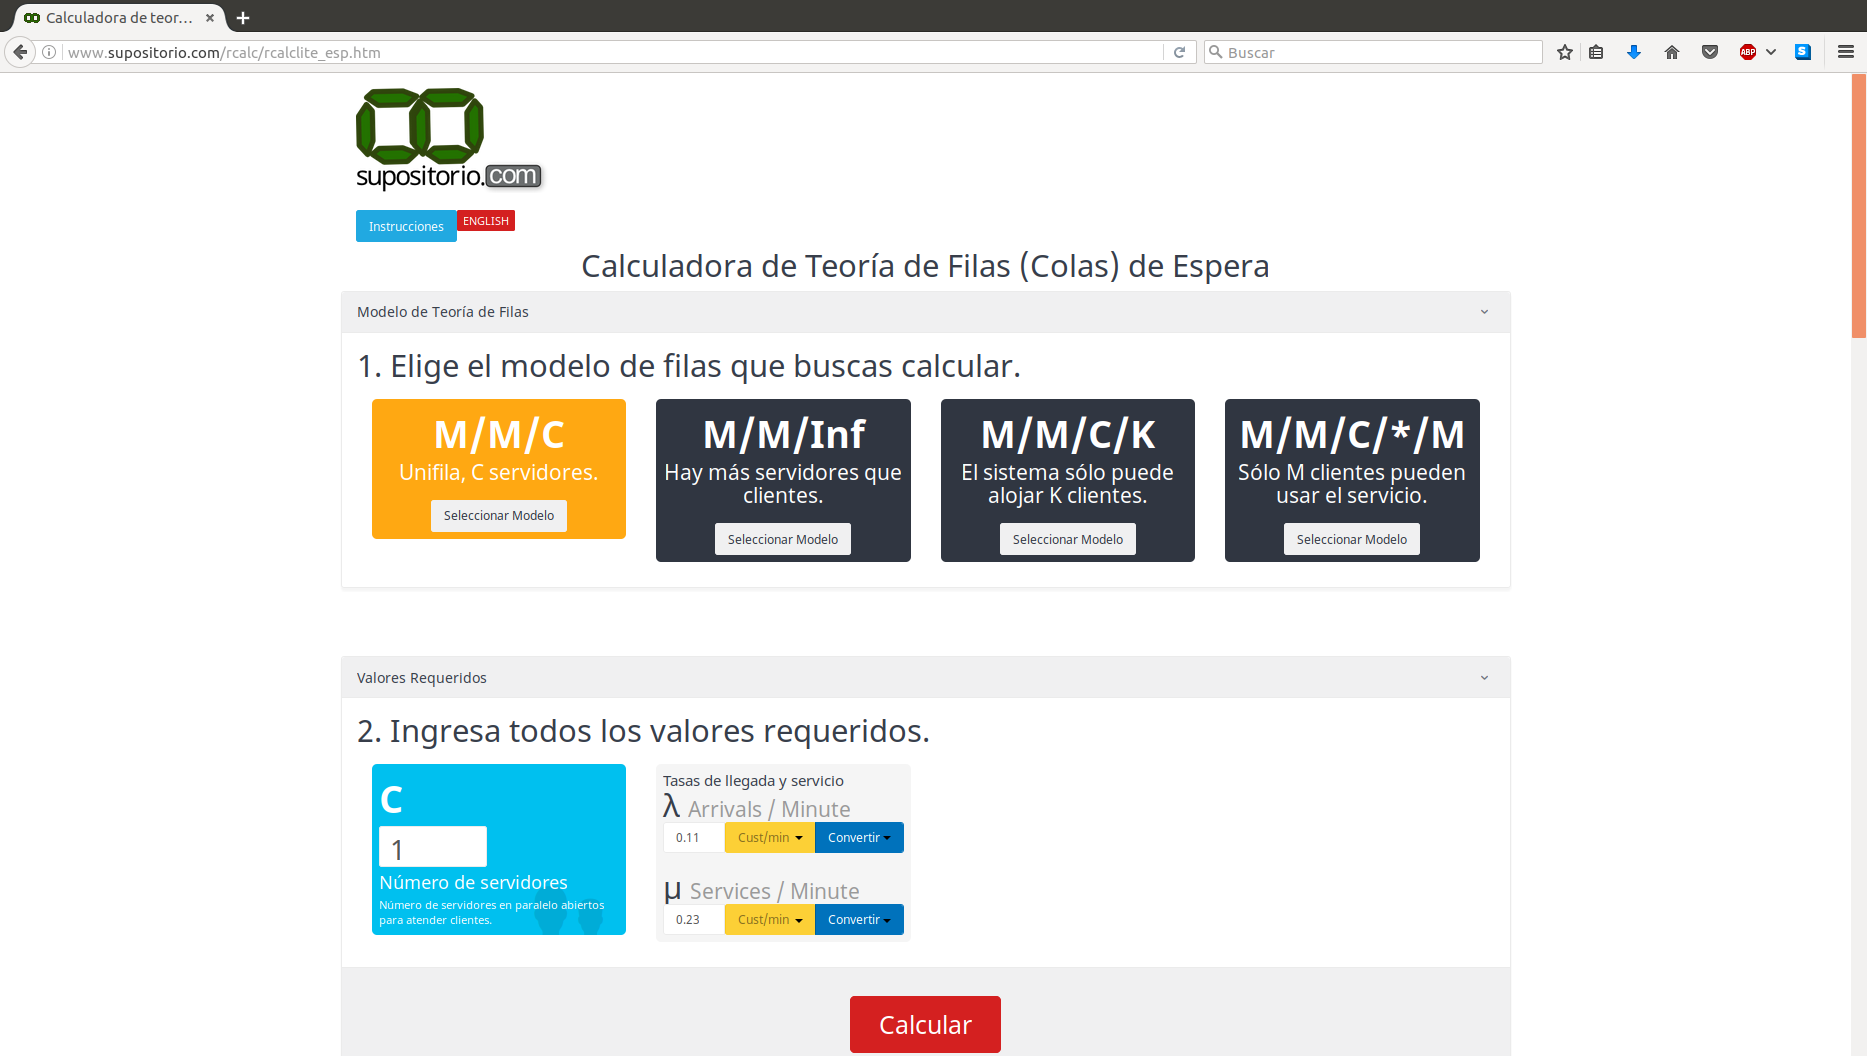
\includegraphics[width=0.6\textwidth]{soft1}
	\label{soft1}
	\caption{Pantalla principal}
\end{figure*}
\newpage
En la pantalla principal de esta página web tenemos una pantalla donde se nos muestran los módelos principales de la teoría de cola. \\
A continuación, por cada modelo, nos pide los parámetros necesarios para calcular las probabilidades de cada modelo, y además, nos muestra gráficas y nos permite calcular probabilidades fácilmente.

\begin{figure*}[h]
	\centering
	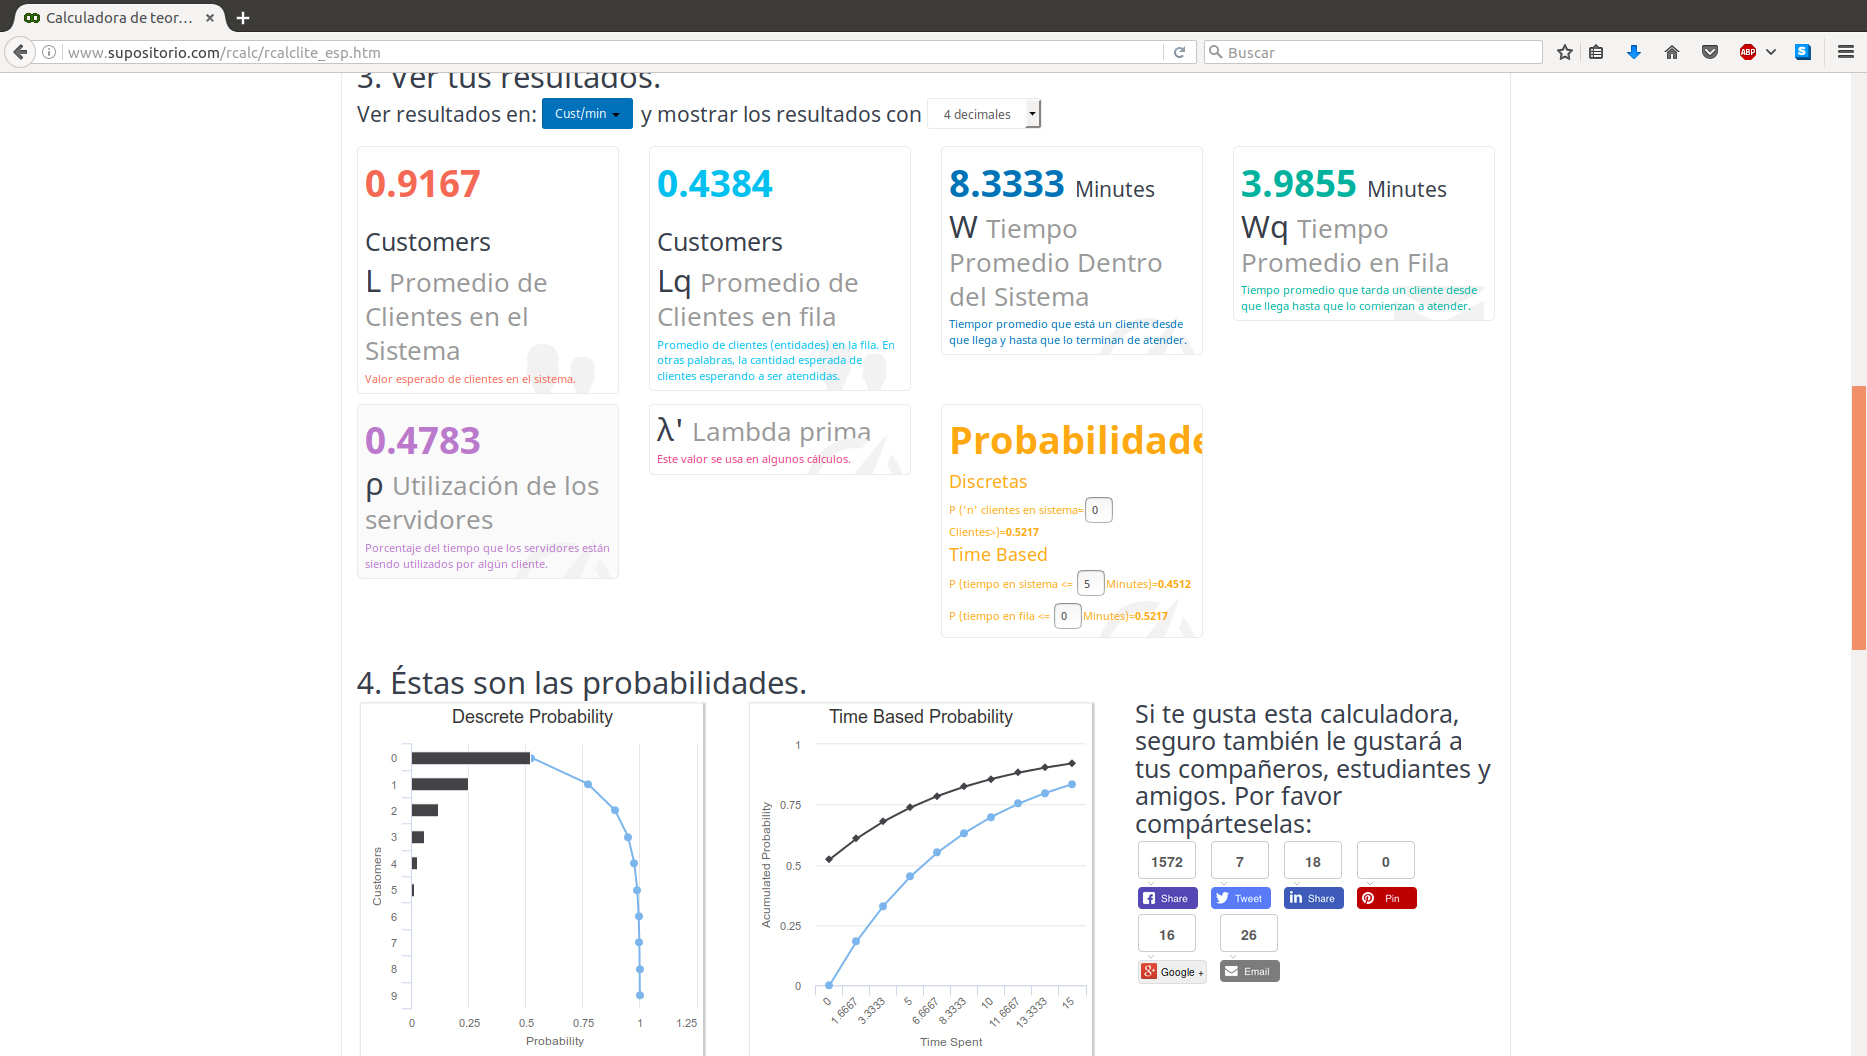
\includegraphics[width=\textwidth]{soft2}
	\label{soft2}
	\caption{Output}
\end{figure*}

Para acceder a este sitio hay que entrar a \href{http://www.supositorio.com/rcalc/rcalclite_esp.htm}{este enlace}, o si lo prefieres escribe en tu navegador: http://goo.gl/DKq59l